\documentclass[11pt]{article}

\usepackage[utf8]{inputenc}
\usepackage[T1]{fontenc}
\usepackage[francais]{babel}
\usepackage{setspace}
\usepackage{fancyhdr}
\usepackage{graphicx}
\usepackage{eurosym}
\usepackage{eso-pic}
\newcommand\BackgroundPic{%
	\put(-1, -302){%
		\parbox[b][\paperheight]{\paperwidth}{%
			\vfill
			\centering
			
\includegraphics[width=40,height=110,%
			keepaspectratio]{ubo_multicolor.png}%
			\vfill
}}}

\title{Rapport projet professionnel \\ Développement logiciel et sécurité informatique}
\author{Thierno Hassane Sow}
\date{\today}

\lhead{}
\rhead{\leftmark}
\begin{document}
	\maketitle
	\AddToShipoutPicture{\BackgroundPic}
\newpage

\pagestyle{fancy}

\renewcommand{\contentsname}{Sommaire}
\renewcommand{\bibname}{Références}

\setcounter{tocdepth}{3}

\tableofcontents
\newpage

	\begin{onehalfspace}
		\section{Introduction}
		\large{
			\begin{it}
		C'était en 2012 quand j'ai pour la première fois vu du code et c'était du HTML. J'avais encore 12 ans à l'époque et je venais de trouver une passion qui était de blogger et en ce temps, j'utilisais Eklablog.\footnote{Système de gestion de contenu (CMS) pas très connu qui sert è faire des blogs gratuitement.} Cette passion m'a petit à petit conduite vers un nouvel univers qui est celui de la programmation. Grâce a Eklablog, je suis rentré en contact avec la programmation et j'ai du commencer avec du HTML\footnote{Langage de description utilisé avec du CSS pour faire le gabarit des sites.}. Durant les deux années suivantes, j'ai appris le CSS, le PHP\footnote{Langage serveur objet très utilisé dans le web.}, le Visual Basic que j'ai vite abandonné et puis le C\#. Grâce à l'excitation que je ressentais en ce moment, j'ai du apprendre beaucoup de langages par la suite comme le C++, le java, le python et le sql avant de comprendre qu'il serait mieux que je me spécialise et j'ai dû choisir le python, le java et le sql pour mes développements. Mon expérience sur tous ces langages me fit comprendre beaucoup de concept comme la programmation orientée objet, les pointeurs en C++ et en C, la communication en parallèles grâce aux threads et en réseaux grâce a python puis la réalisation des tests unitaires. Et encore aujourd'hui je code la plupart du temps, et ce parcours que j'ai du suivre m'a permis de m'investir dans le \begin{bf}développement logiciel et la sécurité informatique\end{bf}.
			\end{it}\newpage
		}


		\section{Matériels et méthodes}
		\subsection{La recherche d'informations}
		Globalement, l'étude que j'ai faite sur les métiers d'ingénieur logiciel et en sécurité informatique s'est réalisée en plusieurs étapes dont: \textbf{la recherche sur le web} à partir des articles, témoignages et ressources multimédias provenant de sites comme celui de l'\begin{bf}Onisep\footnote{Office national d'informations sur les enseignements et les professions}\end{bf} ou sur des documentaires obtenus sur YouTube ensuite par \textbf{interview} d'un spécialiste en développement logiciel puis enfin de mon \textbf{expérience personnelle} acquise au cours de ses cinq dernières années.
		\subsection{Résultats des recherches}
		La phase de recherche a été une expérience à la fois amusante et profitable, elle s'est étalée sur plusieurs jours et s'est conclue par l'obtention de résultats favorables à toutes les questions prévues à cet effet. La majorité de mes réponses proviennent du web. Mes questions se basaient sur les formations à suivre, les débuts dans le secteur professionnel, la journée typique d'un développeur, sa manière d'aborder un projet, les contraintes liées au métier, les possibilités d'évolution qui s'ouvrent à un développeur de logiciels. Concernant mon interview, elle a été faite avec un spécialiste en développement logiciel dans le domaine industriel appelé \textbf{Chris} qui travaille dans la société \textbf{Vetigrasse\footnote{Société spécialisée dans la conception de logiciel dans le domaine industriel}}. Il n'a que sept mois d'expérience dans le domaine et cela m'a été un gros avantage vu qu'il vient tout juste de finir ses études. J'ai obtenu de lui des réponses intéressantes qui ont contribuées à l'élaboration de mon rapport.
		\newpage
		
		\section{Résultats}
		Mes objectifs étant de connaitre le plus possible les métiers d'ingénieurs logiciel et en sécurité informatique, mes recherches m'ont appris beaucoup de choses.
		\subsection{Développement logiciel}
		La phase de recherche s'est répartie en deux phase dont \textbf{les recherches sur le web} et \textbf{l'interview}.
		\subsubsection{Résultats des recherches WEB}
		\begin{description}
			\item[Concernant le travail général d'un ingénieur logiciel: ] il conçoit, produit et assure la maintenance des applications destinées au système d'information d'une entreprise. La réalisation de son projet passe par beaucoup d'étapes notamment l'analyse des besoins du client, le développement du projet avec un langage de programmation, la réalisation des tests puis la rédaction d'une documentation destinée à l'utilisateur \cite{role1}. L'ingénieur en sécurité informatique quant à lui étudie le logiciel, détecte ses points faibles et les neutralisent à travers ses outils tels que: les \textbf{pare-feus} ou des \textbf{modules} destinés à contrer des malwares\footnote{Logiciels malveillants comme les virus et les botnets}\cite{securite}.
			\item[Contraintes liées au métier: ] en général, le métier de développeur est un métier ou l'on est quotidiennement exposé au stress. En effet, il peut arriver qu'ils y'aient des bugs\footnote{Mal fonctionnement d'un programme} qui doivent être résolus dans les plus courts délais, les problèmes liés au temps de développement du produit et celui fixé avec le MOA\footnote{Maitre d'ouvrage ou propriétaire du futur logiciel}\cite{genie_logicie} poussant les développeurs à faire des heures supplémentaires à la maison ou aussi lorsqu'une entreprise décide de changer de voie réduisant ainsi les nombreuses mois de travail fournis aux différents projets qui étaient en cours\cite{contraintes}.
			\item[Pour les possibilités d'évolution qu'offrent le métier,] elles sont diversifiées car un ingénieur logiciel peut travailler dans n'importe quel domaine de la programmation car il est avant tout un spécialiste en développement web et d'applications mobiles par exemple. L'évolution des technologies connectées fait que les concepteurs de logiciels sont de moins en moins exposés au problème du manque d'emploi.
			\begin{figure}[h]
				\begin{center}
					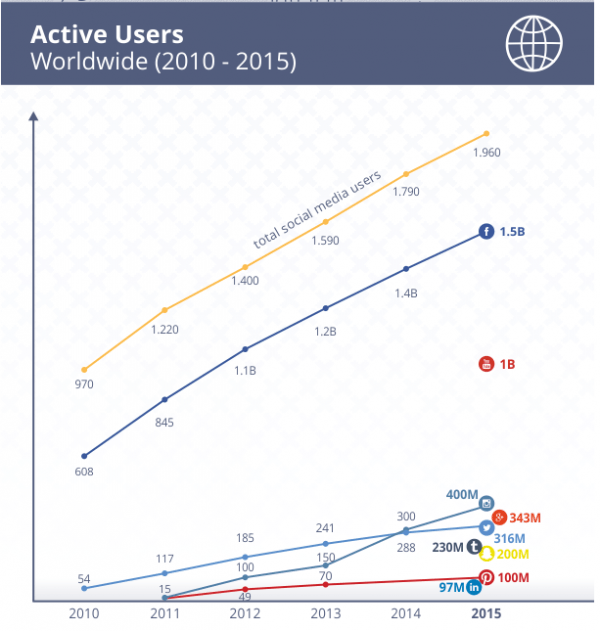
\includegraphics[scale=0.5]{sociaux.png}
				\end{center}
			\caption{L'évolution de la population connectée au fil des années\cite{evolution}}
			\label{L'évolution de la population connectée au fil des années}
			\end{figure}
		\end{description}
		\subsubsection{Résultats de l'interview}
		L'\textbf{interview} m'aura fait comprendre que souvent on est confronté à lire du code écrit par des personnes qui ne respectent pas forcément les mêmes normes de programmation que nous, ce qui est souvent pénible. Malgré qu'on ait obtenu un diplôme, cela ne change rien au fait qu'on doit quotidiennement apprendre et parfois on le fait lorsque l'on a un projet et qu'on doit apprendre une nouvelle technologie pour voir l'implémenter dans le projet. La question qui m'a parue la plus importante est sûrement la première intégration dans le domaine professionnel, évidemment cela est un peu choquant au début de voir un programme avec des dizaines de milliers de lignes de code mais on s'adapte très vite.
		
		\subsection{Et la sécurité informatique ?}
		\subsubsection{Résultats obtenus via documentaire}
		En gros, j'ai appris qu'un jeune pirate de 17-21 ans pouvait avoir entre 8000 et 15000\euro le mois en vendant des numéros de carte bancaire qu'il obtenait en installant des logiciels espions qui enregistrent les numéros de carte chaque fois qu'on les entraient dans un formulaire. Et en général, un pirate a sous son contrôle des centaines de milliers d'ordinateurs ou de téléphones grâce à ses logiciels espions appelés aussi botnets.\cite{pirates} L'ingénieur en sécurité informatique a pour rôle de sécuriser les applications que nous utilisons quotidiennement.
		\newpage
		
		\section{Conclusion}
		\subsection{Conclusion générale}
		La compréhension du métier d'ingénieur en sécurité informatique et logiciel était mon objectif principal, mes recherches m'auront permis de comprendre comment fonctionnait une société de conception de logiciel, comment un développeur informatique vivait sa vie et la partageait avec sa famille et surtout ses responsabilités au sein de son entreprise mais m'aura aussi permis de faire un choix définitif de ma future carrière.
		\subsection{Projection sur l'avenir}
		Le métier de concepteur de logiciels est celui que j'ai toujours souhaité faire et le restera malgré les contraintes liées au métier mais après tout existe t'il un métier sans contrainte ? Donc je continuerai à suivre ma formation actuelle pour j'espère dans le futur pouvoir intégrer une entreprise de conception de logiciel et pourquoi pas diriger une ?
		\newpage
	\end{onehalfspace}
\bibliography{bibli}
\bibliographystyle{plain}
\end{document}          
